\section{上限在软件坐标里的位置}\label{sec:software}

前几节一直以“现实噪声下、输入噪声 $3\times10^{-3}$ 的 31 节点 ESN”为软件对照。这个约定来自把激光强度噪声按调制深度折算到输入（第~\ref{sec:tasks}~节），
但它对结论的影响很大：表~\ref{tab:encodings} 中掩模与 ESN 在 Mackey--Glass 上持平（$3.3\times10^{-4}$ 对 $3.2\times10^{-4}$），
而 ESN 的输入噪声降到 $10^{-3}$ 时为 $5.3\times10^{-5}$，比掩模好约 6 倍，比加了读出侧改进的最好单环也好约 3 倍。
所以本节不取一个点，而是把软件的输入噪声从 0 扫到 $3\times10^{-3}$，把微环放到这条曲线上，回答“一个微环相当于多大、多吵的软件储备池”。

\subsection{软件输入噪声扫描}

图~\ref{fig:software} 给出 31、100、300 节点的 ESN（以及闭环任务中的 NG-RC~\cite{gauthier2021}）的测试误差随输入噪声的变化，协议与微环相同（第~\ref{sec:protocol}~节）；
微环取前几节中最好的结果，画成水平参考线。上方的横轴把输入噪声换算成模数转换器的有效位数：
若满量程对应输入信号的取值范围，$N$ 位量化的噪声均方根为 $2^{-N}/\sqrt{12}$，于是 $10^{-4}$、$3\times10^{-4}$、$10^{-3}$、$3\times10^{-3}$ 分别对应约 11.5、9.9、8.2、6.6 位。

\begin{figure}[htbp]
\centering
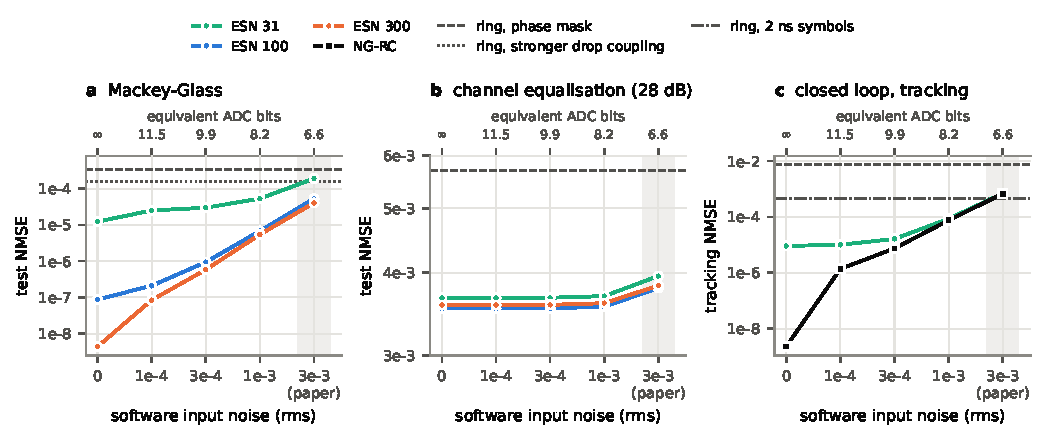
\includegraphics[width=\linewidth]{figS3_esn_input_noise}
\caption{软件储备池的测试误差随其输入噪声（均方根）的变化，上方横轴为等效的模数转换器有效位数 $N$（噪声 $2^{-N}/\sqrt{12}$）。
曲线：31、100、300 节点的 ESN 和 NG-RC（只在闭环任务中）；水平线：现实噪声下的微环（普通谱相位掩模、加大下载端口耦合、$2~\mathrm{ns}$ 符号）。
灰色带为前几节使用的约定值 $3\times10^{-3}$。（a）Mackey--Glass；（b）信道均衡（信噪比 $28~\mathrm{dB}$）；（c）闭环跟踪 Hénon 映射的指令轨迹（补充材料）。
与微环相同的选点和复测流程；Mackey--Glass 为 3 条序列的几何平均，信道均衡除 $3\times10^{-3}$ 外为单条序列，闭环为 4 组训练记录的平均。}
\label{fig:software}
\end{figure}

\emph{Mackey--Glass。} ESN 31 的误差在输入噪声为 0、$10^{-4}$、$3\times10^{-4}$、$10^{-3}$、$3\times10^{-3}$ 时为
$1.2\times10^{-5}$、$2.5\times10^{-5}$、$3.0\times10^{-5}$、$5.3\times10^{-5}$、$1.9\times10^{-4}$；
ESN 100 和 300 在 $3\times10^{-3}$ 时为 $5.3\times10^{-5}$ 和 $4.0\times10^{-5}$，无噪声时为 $8.8\times10^{-8}$ 和 $4.4\times10^{-9}$。
最好的单环（$1.55\times10^{-4}$）与 ESN 31 的交点在输入噪声约 $2.5\times10^{-3}$；100 和 300 节点的 ESN 在整个扫描范围内都更好，在 $3\times10^{-3}$ 时好 3 到 4 倍。

\emph{信道均衡、光纤链路和 NARMA-10。} 前两个任务的误差主要来自信道本身的噪声：ESN 31 的输入噪声从 $3\times10^{-3}$ 降到 0，误差只从 $3.95\times10^{-3}$ 降到 $3.66\times10^{-3}$，
ESN 增大到 300 个节点也几乎不变，但它们在整个扫描范围内都好于最好的微环（$5.7\times10^{-3}$）；
光纤链路上 ESN 为 $1.8\times10^{-2}$，微环最好为 $2.0\times10^{-2}$（补充材料）。
NARMA-10 上，即使在 $3\times10^{-3}$ 时 ESN 31、100、300 也为 $0.11$、$0.041$、$0.032$，好于单环的 $0.19$。

\emph{闭环决策。} 补充材料用微环预测 Hénon 映射的下一步，再按预测值施加有上限的控制。
跟踪一条指令轨迹时，$2~\mathrm{ns}$ 符号的微环跟踪误差为 $4.5\times10^{-4}$；
软件预测器的误差完全由它的输入噪声决定，与微环的交点约在 $2.4\times10^{-3}$，在 $10^{-3}$ 时 ESN 31 和 NG-RC 为 $8.6\times10^{-5}$ 和 $7.5\times10^{-5}$，好约 5 倍。
稳住不稳定平衡点只需要线性反馈，软件的模型能力不是限制，是最干净的标定：交点约在 $1.7\times10^{-3}$。

三个能直接比的任务给出一致的结论：最好的单环相当于输入噪声约 $1.7\times10^{-3}$ 到 $2.5\times10^{-3}$ 的 31 节点 ESN，
按上面的换算约合 \emph{7 位}（6.9 到 7.4 位）有效位数的模数转换器。

\subsection{7 位意味着什么}

这个数字要放在微环能工作的速率下看。本文的微环需要 $Q\sim10^{6}$ 才有足够的 Kerr 非线性，对应约 $0.5$ 到 $1~\mathrm{GBd}$ 的符号率。
这个速率下现成的模数转换器有约 9 位有效位数（例如采样率 $3.2~\mathrm{GSa/s}$ 的 12 位转换器，标称有效位数约 9 位~\cite{ti_adc12dj3200}）；
有效位数降到 5 到 6 位的是 $100~\mathrm{GSa/s}$ 以上、带宽几十吉赫兹的采集系统（例如带宽 $33~\mathrm{GHz}$ 时约 5.9 位、$110~\mathrm{GHz}$ 时约 5.0 位~\cite{keysight_uxr}），而那个速率下微环的 $Q$ 只能取 $2\times10^{4}$ 到 $4\times10^{4}$，Kerr 效应几乎用不上
（补充材料的光纤链路任务中，按 $28~\mathrm{GBd}$ 工作的微环只比线性均衡器好约 15\%）。也就是说，在微环能工作的速率下，把信号数字化后交给 31 节点的软件储备池，精度不会比微环差；
需要微环的场景只能是信号本来就在光域、数字化本身就是要省掉的那一步。

\subsection{读出端也要量化}\label{sec:quant}

上面把软件的输入噪声解读为模数转换器的量化噪声，但微环的 31 路读数同样要数字化，前面的结果都没有计入这一步。
为了让两边对称，我们在最好的单环上给每路读数各接一个 $N$ 位转换器（表~\ref{tab:quant}）。
满量程在拟合用的那次运行上按每路读数的范围标定一次，测试运行沿用这个标定，相当于先校准增益、再固定使用。
考虑两种接法：直接量化光电流的线性转换器，以及在转换器前加对数放大器（等比例的量化台阶，与读出层取对数一致）。
对照是 31 节点的 ESN，它的输入经 $N$ 位量化，不加其他噪声，也就是把软件那一侧的转换器换成真正的量化而不是等效的高斯噪声。

% generated by experiments/make_table3.py; do not edit by hand
\begin{table}[htbp]
\centering
\caption{读出端量化。最好的单环（加大下载端口耦合组，现实噪声，Mackey--Glass）的 31 路读数各接一个 $N$ 位模数转换器，满量程在拟合用的那次运行上按每路读数的范围标定一次，测试运行沿用；“线性”直接量化光电流，“对数”在转换器前加对数放大器。对照是输入经 $N$ 位量化、不加其他噪声的 31 节点 ESN（一个随机储备池）。3 条序列 $\times$ 6 对新运行的几何平均。不量化时微环为 $1.5\times10^{-4}$，无噪声的 ESN 为 $2.4\times10^{-5}$。}
\label{tab:quant}
\small
\begin{tabular}{cccc}
\toprule
位数 $N$ & 微环，线性转换器 & 微环，对数放大器 & ESN 31，输入量化 \\
\midrule
4 & $4.2\times10^{-3}$ & $1.9\times10^{-3}$ & $3.5\times10^{-3}$ \\
5 & $2.2\times10^{-3}$ & $1.1\times10^{-3}$ & $1.3\times10^{-3}$ \\
6 & $1.2\times10^{-3}$ & $5.6\times10^{-4}$ & $4.5\times10^{-4}$ \\
7 & $6.0\times10^{-4}$ & $3.5\times10^{-4}$ & $2.3\times10^{-4}$ \\
8 & $3.6\times10^{-4}$ & $2.7\times10^{-4}$ & $1.3\times10^{-4}$ \\
9 & $2.7\times10^{-4}$ & $2.1\times10^{-4}$ & $9.3\times10^{-5}$ \\
10 & $2.0\times10^{-4}$ & $1.8\times10^{-4}$ & $6.8\times10^{-5}$ \\
12 & $1.6\times10^{-4}$ & $1.6\times10^{-4}$ & $4.6\times10^{-5}$ \\
\bottomrule
\end{tabular}
\end{table}


微环需要较多的位数才不被量化拖累：两种接法都要 10 位，误差才回到不量化时（$1.54\times10^{-4}$）的 1.3 倍以内；
到 7 位时分别为 $6.0\times10^{-4}$ 和 $3.5\times10^{-4}$，差 2 到 4 倍。
原因在于梳齿功率跨越几个数量级，线性转换器分给弱梳齿的台阶很少；对数放大器缓解了这一点，但没有消除。
在 6 到 12 位的每一档，输入经同样位数量化的 ESN 都比 31 路都量化的微环好 1.2 到 3.4 倍（与带对数放大器的微环比；与线性转换器比差得更多）；
只有在 4 和 5 位这样很粗的量化下，带对数放大器的微环才好于 ESN，而那里两者的误差都在 $10^{-3}$ 以上。
另一个读法是：不量化的微环（$1.54\times10^{-4}$）落在输入量化 7 到 8 位的 ESN 之间（$2.3\times10^{-4}$ 和 $1.3\times10^{-4}$），与上一小节按等效噪声换算的约 7 位一致。

所以补上读出端的量化以后，比较只对微环更不利：软件只需要在输入端放一个转换器，而微环要 31 个，每个还要有约 10 位的有效位数。
在 $1~\mathrm{GBd}$ 下这样的转换器可以做到，但 31 路的功耗和成本是实际的代价。
如果在光域完成加权（用谱整形器加平衡探测直接算出读出层的线性组合），就只需要一个转换器；但延迟抽头这时要用光延迟线实现，本文没有模拟这种读出。

\subsection{多环阵列的上限}

单环的误差约一半来自它自己的失谐抖动和散粒噪声（第~\ref{sec:noise}~节），这两项在不同的环之间是独立的。
几个掩模不同的环共用一个输入光梳、读出拼接（每环 31 根梳齿 $\times$ 8 个抽头）时，这部分噪声会被平均掉。
训练长度加到 16 倍（16320 个符号）后，加大下载端口耦合的 1、2、4、8、16、32 个环为
$1.27\times10^{-4}$、$3.4\times10^{-5}$、$1.36\times10^{-5}$、$8.4\times10^{-6}$、$6.7\times10^{-6}$、$6.9\times10^{-6}$，
16 个环后不再下降，即误差降到单环的约 1/19 后饱和。
让所有环共用同一份激光强度噪声（同一个输入光梳分给所有环），结果几乎不变（16 个环为 $6.8\times10^{-6}$），说明饱和不是来自共模的光源噪声。
同样训练长度下，输入噪声 $3\times10^{-3}$ 的 ESN 100、300、1000 为 $3.9\times10^{-5}$、$2.1\times10^{-5}$、$1.4\times10^{-5}$，阵列好 2 到 3 倍；
但输入噪声降到 $10^{-3}$ 时（一条序列）为 $6.8\times10^{-6}$、$3.2\times10^{-6}$、$1.65\times10^{-6}$，100 节点的 ESN 已与 16 个环持平，1000 节点好约 4 倍。
所以阵列也只是把上限在软件坐标里往右移了一些，没有改变结论。
多环只在任务受各环自身噪声限制时有用：信道均衡在 $28~\mathrm{dB}$ 的信道噪声下加环和加大 ESN 都没有改善。

\subsection{为什么 $3\times10^{-3}$ 的约定偏严}

$3\times10^{-3}$ 是把激光强度噪声（$10^{-3}$）除以调制深度（$0.33$）得到的，相当于假设软件的输入和微环的输入一样吵。
但这一项在微环里的影响很小：第~\ref{sec:breakdown}~节中只打开激光强度噪声时，微环的误差只升高 1.5 到 1.9 倍；
而 ESN 31 在输入噪声 $10^{-4}$ 时就已经升高 2 倍。同一份强度噪声，对微环的伤害远小于把它折算成输入噪声后对 ESN 的伤害
（原因可能是强度噪声在微环里同时作用于泵浦和所有输入梳齿，部分表现为共模的变化，我们没有单独验证）。
所以 $3\times10^{-3}$ 对软件偏严，前几节中“与 ESN 31 持平”的说法都应理解为在这个偏严的约定下成立；
更公平的比较点在 $10^{-3}$ 附近，那里软件在本文的每个任务上都更好。

这一节的结论是：\emph{在本文考察的任务上，Kerr 微梳储备池的精度上限低于同规模的软件储备池；单个微环相当于输入接约 7 位模数转换器的 31 节点 ESN}。
评估协议是这个结论的一部分：只看一次噪声实现会乐观 10\% 到 30\%，混沌区的结果不可重复，给软件设的输入噪声能让比较翻转，所以我们给出整条曲线而不是一个点。
